\item Find the accelerations of rod $A$ and wedge $B$ in the arrangement shown in Fig. 1.20 if the ratio of the mass of the wedge to that of the rod equals $\eta$, and the friction between all contact surfaces is negligible.
    \begin{center}
        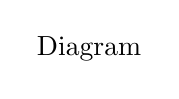
\begin{tikzpicture}
            \node at (0, 0) {Diagram};
        \end{tikzpicture}
    \end{center}
\begin{solution}
    \begin{center}
        \begin{tikzpicture}
            \pic at (0, 0) {frame=3cm};
        \end{tikzpicture}
    \end{center}
    
    \begin{align*}
        \intertext{Let us draw free body diagram of each body, i.e., of rod $A$ and of wedge $B$ and also draw the kinematical diagram for accelerations, after analysing the directions of motion of $A$ and $B$. The kinematic relationship of accelerations is}
        \tan \alpha &= \frac{w_A}{w_B} \tag{1}
        \intertext{Let us write Newton’s second law for both bodies in terms of projections having taken positive directions of $y$- and $x$-axes as shown in the figure:}
        m_Ag - N \cos \alpha &= m_A w_A \tag{2} \\
        N \sin \alpha &= m_B w_B \tag{3}
        \intertext{Simultaneous solution of Eqs. (1), (2) and (3) yields}
        w_A &= \frac{m_A g \sin \alpha}{m_A \sin \alpha + m_B \cot \alpha \cos \alpha} = \frac{g}{(1 + \eta \cot^2 \alpha)} \\
        \intertext{and}
        w_B &= \frac{w_A}{\tan \alpha} = \frac{g}{(\tan \alpha + \eta \cot \alpha)}
    \intertext{Note: We may also solve this problem using conservation of mechanical energy instead of Newton’s second law.}
    \end{align*}
\end{solution}
